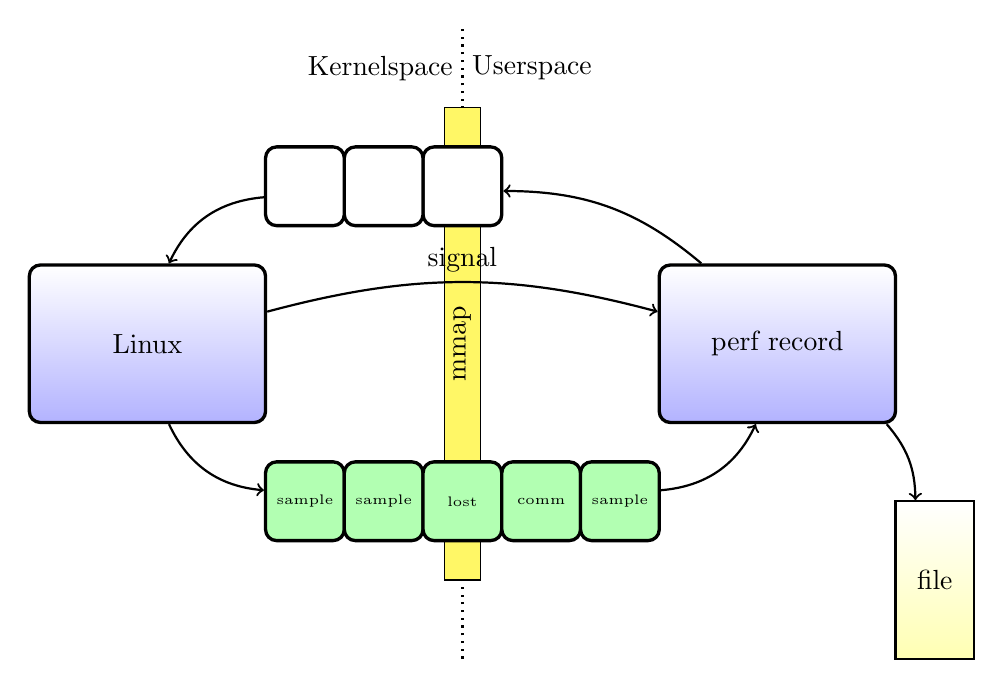
\begin{tikzpicture}[scale=1,transform shape]
\tikzstyle{app}=[anchor=center,minimum width=3 cm,minimum height=2 cm,rectangle,rounded corners,draw=black, top color=white, bottom color=blue!30,very thick, text centered]
\tikzstyle{map}=[anchor=center,minimum width=1 cm,minimum height=1 cm,rectangle,rounded corners,very thick, text centered,draw=black,fill=white]
\tikzstyle{event}=[map, fill=green!30,very thick, text centered]
\tikzstyle{arrow}=[->,thick]
\tikzstyle{Interface}=[rectangle,draw=black, fill=yellow!60,rotate=90]
\tikzstyle{file}=[anchor=center,draw=black, top color=white, bottom color=yellow!30,thick, text centered]


\path [thick, dotted] (0,-4) edge (0,4);
\node [anchor=east] at (0,3.5) ()  {Kernelspace};
\node [anchor=west] at (0,3.5) ()  {Userspace};
\node [Interface,minimum width=6 cm] at (0,0) (iface) {mmap};

\node [app] at (-4,0) (linux)  {Linux};
\node [app,minimum width=3 cm,minimum height=2 cm] at (4,0) (perf)  {perf record};

\path [arrow,bend right=-15] (linux) edge node[above]{signal} (perf);

\node  [event] at (-2,-2) (ev0) {\tiny{sample}};
\node  [event] at (-1,-2) (ev1) {\tiny{sample}};
\node  [event] at ( 0,-2) (ev2) {\tiny{lost}};
\node  [event] at ( 1,-2) (ev3) {\tiny{comm}};
\node  [event] at ( 2,-2) (ev4) {\tiny{sample}};

\path [arrow,bend right=30] (linux) edge (ev0);
\path [arrow,bend right=30] (ev4) edge (perf);

\node  [map] at ( 0, 2) (ev5) {};
\node  [map] at (-1, 2) (ev6) {};
\node  [map] at (-2, 2) (ev7) {};

\path [arrow,bend right=20] (perf) edge (ev5);
\path [arrow,bend right=30] (ev7) edge (linux);

\node [file,minimum width=1 cm,minimum height=2 cm,rectangle] at ( 6, -3) (file) {file};
\path [arrow,bend right=-20] (perf) edge (file);
\end{tikzpicture}
